\section{Smart Cities \& Urban Informatics}
Urban Analytics and Informatics is a relatively new, multidisciplinary, and broad field of research that contributes to identify, describe and solve urban challenges. Its name indicates the conjunction of two disciplines. On one hand, brings specific knowledge from economics, sociology, or geography to address urban dynamics such as gentrification, segregation, lack of accessibility or housing informality. On the other hand, uses a quantitative approach to understand these dynamics. Urban analytics focuses on many domains but uses a specific toolbox to explore these topics. \par
Michael Batty, founder of the Center of Advanced Spatial Analytics (CASA) at UCL defines it as a 
\begin{quote}
    fast emerging as the core set of tools employed to deal with problems of big data, urban simulation, and geodemographics
\end{quote}
In another quote, Professor Emeritus of Geography at Santa Barbara University, Michael Goodchild, describes it as a 
\begin{quote}
New kind of urban research, one that exploits the vast new data resources that are becoming available from social media, crowd sourcing, and sensor networks (...)
\end{quote}
\cite{singletonUrbanAnalytics2018}. \par

During the last past years, a set of new forms of data and computational approaches have enabled a New Science of Cities to raise. But as the old KPIS, these new data sources do not produce insights on their own. Data needs to be stored, cleaned and combined with different sources to be used. Urban Analytics is the disruptive approach that enables to handle big quantities of information to answer urban questions. Among the toolbox often employed we could list: (i) Modelling, (ii) Visualization, (iii) Data Capture, (iv) Data Science, (v) GIS and (vi) Simulations. \par

In order to illustrate what Urban Analytics and Informatics is capable of, a set of four projects are described below. Although, in each project different features of the toolkit are used, the strongest and most innovative resource was highlighted. 


\subsection{Data Science}
In this example, Google Street View is used to create a perception index of how green a city is. In opposition to using satellite images or tree census, the objective of this project is to capture the amount of perceived green by the citizens of a settlement. Besides the innovative use of an already existing data source, the project is data intensive, as the images need to be processed and determine the amount of greenery.
\url{http://senseable.mit.edu/treepedia}




\subsection{New Data Sources}
The second case tries to tackle one of the mayor data limitations faced by planners, politicians or any other stakeholder of the city. Using the data of a food service application the project managed to estimate the amount of people that lived in different cities in china. The results produced a more detailed dataset of the population (temporal and spatial) than what an official census can provide.
\url{http://senseable.mit.edu/tasty-data/}

\subsection{Data Capture}
In some cases, Urban Analytics and Informatics can contribute to create a new data set. In this opportunity small trackable devices are embedded in objects to be thrown away. As a result, the, spatial-temporal trace of waste is generated. There is a completely new data set of where the waste is generated, where did it traveled and for how long and where it ended. 
\url{http://senseable.mit.edu/trashtrack/}




\subsection{Visualizations}
Another important component of Urban Analytics is to summarize the findings and highlights of big and complex data sets in a comprehensible way. Using an adequate visual strategy is important to make the results of the research understandable by a specific audience. In this opportunity GeoFluxus, was selected as an example as the project objective is to map and visualize the flow of waste.
\url{http://geofluxus.com/#data}


\begin{figure}[H]
    \begin{multicols}{2}
    \noindent
    \subfloat[Data Science]{\centering
    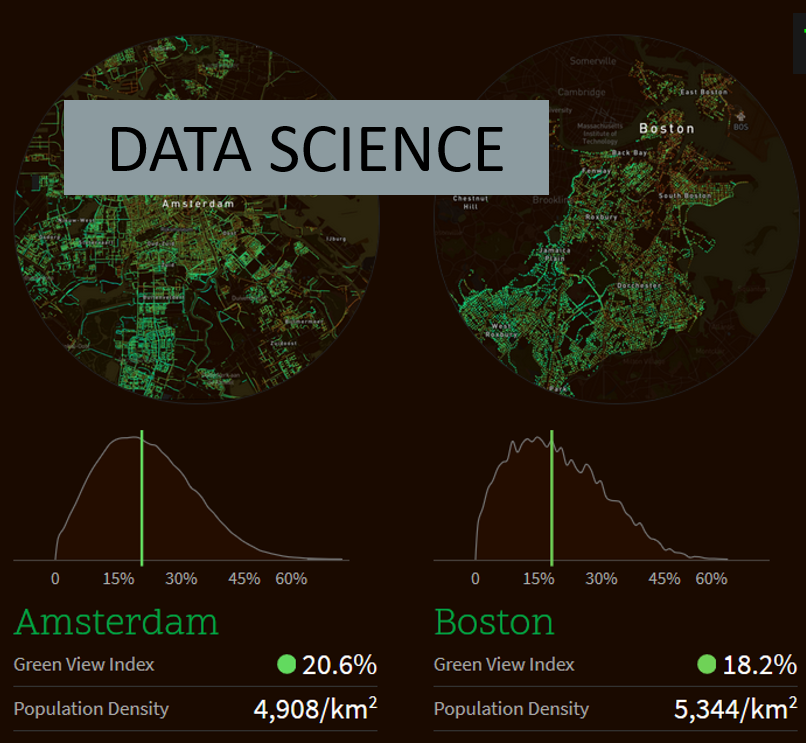
\includegraphics[width=0.9\linewidth, height=6cm]{Imgs/4_ds.PNG}}\par 
    %
    \subfloat[New Data Sources]{\centering
    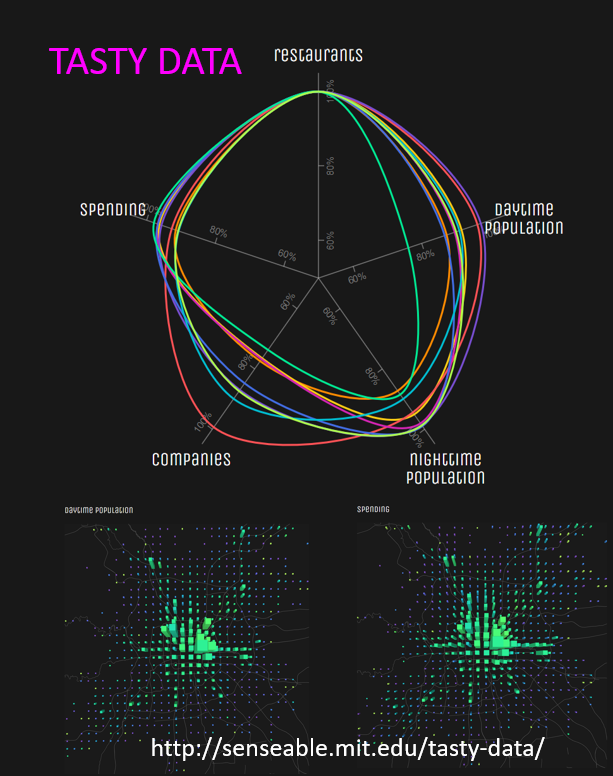
\includegraphics[width=0.9\linewidth,height=6cm]{Imgs/5_new_data.PNG}}\newpage
    %
    \subfloat[Data Capture]{\centering
    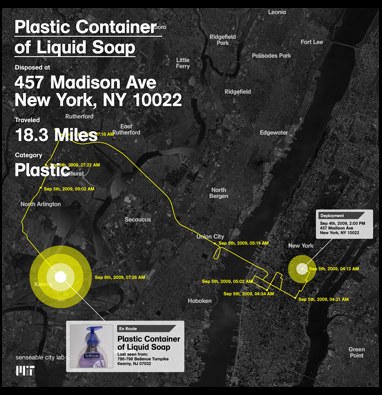
\includegraphics[width=0.9\linewidth,height=6cm]{Imgs/6_trash_track.PNG}}\par
    %
    \subfloat[Visualization]{\centering
    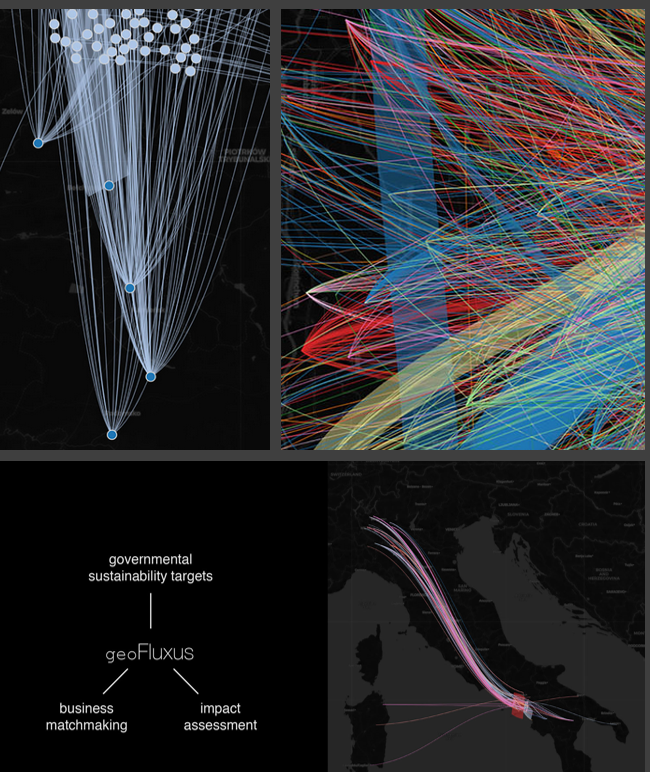
\includegraphics[width=0.9\linewidth, height=6cm]{Imgs/7_flux.PNG}}
    %
    \end{multicols}
    \caption{Urban Analytics and Informatics toolkit}
    \label{UA_toolkit}
\end{figure}